
% to choose your degree
% please un-comment just one of the following
\documentclass[bsc,frontabs,twoside,singlespacing,parskip,deptreport]{infthesis}     % for BSc, BEng etc.
% \documentclass[minf,frontabs,twoside,singlespacing,parskip,deptreport]{infthesis}  % for MInf


\usepackage{graphicx}
\begin{document}

\title{Implementing an online open-source prediction market framework}

\author{Yordan Stoyanov}

% to choose your course
% please un-comment just one of the following
%\course{Artificial Intelligence and Computer Science}
%\course{Artificial Intelligence and Software Engineering}
%\course{Artificial Intelligence and Mathematics}
%\course{Artificial Intelligence and Psychology }   
%\course{Artificial Intelligence with Psychology }   
%\course{Linguistics and Artificial Intelligence}    
%\course{Computer Science}
\course{Software Engineering}
%\course{Computer Science and Electronics}    
%\course{Electronics and Software Engineering}    
%\course{Computer Science and Management Science}    
%\course{Computer Science and Mathematics}
%\course{Computer Science and Physics}  
%\course{Computer Science and Statistics}    

% to choose your report type
% please un-comment just one of the following
%\project{Undergraduate Dissertation} % CS&E, E&SE, AI&L
%\project{Undergraduate Thesis} % AI%Psy
\project{4th Year Project Report}

\date{\today}

\abstract{
Model aggregation, markets, prediction markets.

My market
}

\maketitle

\section*{Acknowledgements}
You guys have been a great inspiration!

\tableofcontents

%\pagenumbering{arabic}


\chapter{Introduction}

Information has been traded extensively in one way or another since the dawn of man. While true, this fact has become increasingly relevant in recent years with advances such as the information economy and big data transforming the way we think about data and the knowledge it implies \cite{mcgee_managing_1993}; at the same time it has never been harder to quantify its value.


The problem of efficiently combining information coming from different sources in order to form a rational belief is largely an unsolved issue in Bayesian philosophy \cite{greene_collective_2010}. It manifests in the domain of machine learning as the problem of belief aggregation which deals with the design of algorithms that combine the beliefs of multiple learners in order to elicit a more reliable prediction. In practice though existing solutions are far from ideal in the sense that they do not provide flexible enough methods of combining the different beliefs of different (heterogeneous) sources into a uniform output. 

    If we take a look at ordinary commodity trading though it is apparent that the existence of a market where agents exchange goods using a common currency provides a meaningful way to determine the prices of the traded goods. Note that while the traded goods can be physical, it is often the case that they are purely conceptual. For example the prices of stock market shares reflect the public's expectation of the performance of a company in the near future. The basic market needs not be active with regard to the traded goods and is in principle nothing more than the market squares that have existed in towns for ages. In its essence a market provides the basic process for determining the price, demand and ownership of various goods or services.

    A prediction market is a special kind of a market which allows agents to trade on and share their information on a future event with the public. This is achieved by creating a market where the trading goods are akin to shares corresponding to each of the possible outcomes of the events of interest. Each share promises a fixed payment in the future to its holder if and only if the outcome associated with it happens to be the event's actual result. This future point is usually fixed at the start of each challenge, necessarily after the result of the event has been observed by the public. In such a way players are incentivised to trade on the difference between their beliefs and those of the market: rational agents would buy shares at what they perceive to be a lower price as this increases their expected profit. By doing so they practically inform the market and the public of their knowledge and help establish the equilibrium price.

    Another possible application of prediction markets deals with the creation of crowdsourced machine learning competitions. Such challenges are becoming increasingly popular in recent years.. A prominent example is the {\em Netflix prize} challenge which was held as early as 2006 with the goal of improving the classification algorithms used by the company \cite{bennett_netflix_2007}. The online platform {\em Kaggle} takes a slightly different approach by instead hosting such competitions on the behalf of third parties. 
    
The main motivation behind such approaches is to leverage the knowledge of the public at scale by offering incentives for the interested and knowledgeable parties. Although fairly successful, [cite?] existing approaches do exhibit a few shortcomings: most notably, they are inherently anti-collaborative                                                                                                                                                                                                                                                                                                                                                                                                                                                                                                                                                                                                

    My project deals with the implementation of a flexible online prediction and machine learning market framework. In contrast to existing solutions, it is mostly intended as a clean and extensible platform to be used as a base for further efforts. To this end the software offers a concise, well-tested and documented prediction market core with a modular architecture which allows for the creation and experimental comparison of different pricing algorithms. Being a web platform it has a full-featured though fairly unsophisticated user interface, but also includes a comprehensive user-facing API which permits and encourages algorithmic trading.
   
   
   
\chapter{Definitions}

    In this section I outline existing approaches to the problem of model aggregation, introduce the concept of prediction markets, and finally talk about their use in a machine learning context. 
% Define markets, prediction markets. Detail how we use them to aggregate beliefs.


\section{Model Aggregation}
    In machine learning the problem of model or belief aggregation deals with the design of meta-algorithms that use a number of existing classifiers for a specific task in order to elicit a more accurate prediction than any of the constituent algorithms. Such algorithms are called {\em ensemble methods} [TODO: few more sentences about ensemble methods, examples]

\section{Market}

    Markets provide a common ground for the exchange of goods between different agents. Basic markets are neutral towards both the participants and the goods being traded and do not have the concept of currency which is seen as another good instead. Each of the agents has an associated {\em position} in each of the goods being traded in the market which is simply the amount of the good they currently possess. In general, there is no restriction on the value of the agent's position and we will distinguish between {\em long positions} where the agent has a positive holding, and {\em short positions} where the agent has a negative amount of the good.

    A basic model of such a market is the {\em order book} which records and matches the bids and offers placed by participating agents. Such a market is {\em neutral} with regard to the goods as it never owns any. Note that there is an inherent degree of freedom when implementing the matching process: arbitrage opportunities must be dealt with care if the market is to be strictly neutral, and the same goes for partially completing orders (since rarely, if ever both the price and the quantity will match).


\section{Prediction Market}

    A prediction market is a type of market with an agreed currency where each of the remaining goods is tied to exactly one of the possible outcomes of a future event. Each good promises a fixed reward (taken to be 1 credit for simplicity) in case the outcome associated with it happens to be the event's actual result, and zero otherwise. Goods can be additionally created by agents for sale, which is equivalent to the agent assuming a short position in the market.
    
    Prediction markets have been shown to outperform other traditional forms of prediction such as polls. They have been used with success in the past for health care (Polgreen et al. 2006), to aid decision-taking in large corporations (Cowgill et al., 2008), and to predict presidential elections (Dudik et al., 2012). Recently prediction markets such as intrade.com were also shown to provide more accurate results on the Scottish referendum as compared to traditional voter polls \cite{bell_the_2014}.


\section{Machine Learning Market}
    Machine learning markets are a fairly recent extension of the concept of prediction markets which establish significant parallels between prediction markets and existing machine learning approaches for model combination. In a machine learning market the players are machine learning agents possessing individual utility functions and probabilistic beliefs. 
 
\section{Market Maker}
    Wat?

\chapter{Related Work}

I will then review some case studies of prediction markets at work. Finally I will have a look at the existing solutions that could be used as a base for my project.

\section{Existing Software}
%
    My search for software started first and foremost with an investigation of the open-source solutions which could be used as a starting point for my project. I then had a look at a number of closed-source or commercial prediction markets which I investigated similarly in terms of UI and functionality.   
    
\subsection{Open source}
    Despite the fact that prediction markets are not a particularly novel concept and are relatively well-studied I was unable to find a satisfying project which I could use as a starting point for my project/ market?). The solutions I found and examined were in general too limited in architecture, mostly outdated and built on top of aging or relatively uncommon web stacks.

\begin{itemize}

\item {\tt Zocalo}

    Zocalo is an MIT-licensed prediction market written in Java using Java Server Pages (JSP) and Hibernate. It is probably the most prominent of the listed examples having been used in a number of research projects already [cite?]. It allows the creation of both {\em order book} and {\em market maker}-based markets of a single discrete variable. While it uses AJAX to implement updates in real-time, the user interface is fairly simple as it is rendered (or stitched) on the fly using Java strings. This and the fact that the code-base is already large and tightly coupled means it may be difficult to extend or modify existing parts of the software. There is also no public market API and writing one in addition to supporting multivariate markets could prove hard due to the aforementioned reasons.

\item {\tt ideafutures } \footnote{http://ideafutures.sourceforge.net/}

    {\tt Ideafutures} seems to be one of the first online prediction markets in existence dating as far back as 1995. It has been featured in a number of publications (cite). It only supports only markets of single binary variables and offers a fairly simplistic, textual interface.

Although it is used by at least one operating market (the play-money Foresight Exchange) development on the software seems to have stopped since 2005. It is additionally written in Perl and uses BerkeleyDB (as opposed to a traditional database) which makes it less of an ideal choice.

\item {\tt Open Prediction Markets}

    Drupal is a modular, open-source content management system written in PHP and {\tt Open Prediction Markets} is a module which implements prediction market functionality on top of it. The only market types that are  supported are {\em parimutuel} markets of single discrete variables. Its interface is similarly textual and does not seem to reflect changes in real-time.
    
    Although considerably more recent than the other examples in this list, the {\tt Open Prediction Markets} module is nonetheless far from an ideal base for my project due to its limited functionality and choice of language.
    
\end{itemize}

\subsection{Commercial}
    Of note is also the presence of a number of commercial or simply closed-source prediction markets that could be used as a point of reference in terms of features and model flexibility. Due to the fact that markets dealing in financial securities are regulated in many parts of the world, most of the markets I looked at use alternative currencies such as Bitcoin. 
    
\begin{itemize}

\item {\tt Betfair}

    [TODO: a betting platform or a prediction market? betfairpredicts-dot-com and the UK general election]
    
\item {\tt bitbet.us}

    BitBet is a website where participants can use Bitcoin to play in parimutuel markets of binary outcomes. Thanks to the simple market mechanism its interface and betting process are fairly streamlined with intuitive visualisations and registration-free betting using Bitcoin and QR-codes. While it is not strictly a prediction market as it doesn't deal with securities, it shines mostly for the minimalistic and clean user experience it offers.

\item {\tt Predictious}

    Similarly to the previous example this website uses Bitcoin and supports only markets of binary variables. It is also a proper prediction market albeit entirely passive: there is no market maker and an order book is instead used.

    While simple in terms of market structure, the user interface of {\tt Predictious} is considerably more varied and includes price and activity histograms, as well as views of the outstanding orders specific to a given market or a player.


\item {\tt Fairlay} 

    [TODO: another bitcoin exchange. worth it?]

\end{itemize}


\chapter{Project Scope}
    Here I outline the scope of the project in terms of the major milestones that I accomplished.



\section{Accomplished Goals and Milestones}    

\subsection{Design a simple, expressive prediction market framework}
    % talk about bduf, agile and finance software needs 2 be reliable
    This involves modeling the market-player relations from the market maker’s view in a structured and sane fashion. [TODO: clarify]

Allow the placing of orders (bets) using a human-facing web interface and market management using simple Python commands or an admin interface. It should be possible to track and advance challenges (representing the true results for the current iteration) in a market, and raise events to announce the arrival of orders and challenge progression to the corresponding market maker modules. 

\subsection{Develop a modular market maker architecture}

Market makers control the prices and exchange of goods in the market. They are thus vital to the predictive performance of the resulting information market. A flexible prediction market framework 




\subsection{Write a simple, functional user interface}
    The user interface is arguably one of the most important aspects of the software when it comes to player engagement. While it should necessarily provide basic functionality in terms of market interactions, such as observing and participating in a market, [it should also be informative, non-misleading, and in real-time]. 
On the other hand UI is one of the actually {\em lesser} goals in terms of project. I had little to no experience in writing web front-ends when I started working on the project although I had some specific ideas in mind (see Future Work). In the end I would leave the UI extensions or perks for the final stage of the project. 
    
    The final user interface nonetheless provides the major functionality expected of an online trading platform: it provides market listings, registration and detailed views and forms for placing and canceling orders. These features are built on top of the user authentication module that is part of the default Django installation and provides the basic means for user registration and session management. Although it is static as it does not reflect market changes in real-time, adding support for real-time updates to the user interface should be fairly straightforward.
    

\subsection{Allow programmatic access}
    The ability to use an API in order to manage and interact with the prediction markets would allow the execution of experiments where some or all of the participants are automated. In light of recent studies (see Chapter 4) such a tool could be used to experimentally establish equivalences between particular market setups and machine learning techniques. As it can be also utilised by ordinary market players

    An important consequence of the aforementioned  feature will be the possibility to run prediction markets where players are encouraged to write their own machine learning algorithms in order to beat the problem at hand. While there are existing platforms that deal with the same problem of designing a machine learning classifiers using crowdsourcing (e.g. {\tt kaggle.com}), they do so in an inherently competitive (and thus non-collaborative) winner-takes-all model. In contrast prediction or machine learning markets allow the elicitation of beliefs based on the performance of {\em all} of the participating agents.
    
    
\subsection{Implement a number of sample market makers}
I will look in detail at algorithms for price formation in prediction markets including scoring-rule based ones, parimutuel betting schemes, but also more involved models which establish clearer connection between the actions of traders and their underlying beliefs. observed prices and the underlying probability of outcomes such as the ones described by Barbu and Lay [cite?]

\section{Future Work}

\subsection{Implement an intuitive and dynamic market UI}
    Although complete in terms of functionality, there are some areas where the current user interface is lacking.
    
    Its most noticeable drawback is the lack of real-time updates that reflect changes of the market state. While such a functionality could be implemented in a straightforward manner using AJAX or WebSockets, my limited experience with JavaScript dictated my decision to leave this feature as optional. 
    
    A related issue is the fact that the present user interface is overly textual and lacks informative visualisations. Although I intended to include simple, even static, market and activity histograms, this ended up being more involved than I anticipated. After I struggled for a while with various JavaScript graphics frameworks and JSON formatters I ultimately decided I would rather complete the functional part first.  

\subsection{Allow event composition and relation}

    Even though the current architecture properly supports multivariate markets of discrete variables, it accomplishes this by treating all of the dimensions as independent from each other. While this assumption is generally sound and may be close enough to the truth in practical examples, improving the market design by e.g. allowing the creation of event pairs or triples is a necessary step towards the creation of a flexible prediction market framework. A similar approach is described in [cite]. 
    

\chapter{Implementation}

    This chapter details the design decisions taken while building the project. I first talk briefly about the technologies I decided to use and why I started from scratch instead of extending an existing one. I then continue by examining existing software stacks in terms of how suitable the language and libraries are for the task at hand. Finally I outline the major architectural components of the completed project and the ways they interact with each other.

\section{Design}

    When approaching the project one of my main goals was to build a software which could be both used and extended easily. On the other hand the specific nature of the project - financial prediction markets - means that it should be easy to both understand and verify the correctness of the code. These two goals are inherently clashing: [TODO]
    
With this in mind I explored the following choices of programming platforms:

\begin{itemize}
\item Python

Python is a popular dynamic language supporting a number of programming paradigms. In addition to its comprehensive standard library there is a variety of available packages that cover a wide range of functionality notably in terms of web development. Django\footnote{https://www.Djangoproject.com/} is a popular full-stack framework which supports a number of database back-ends and emphasises modularity and readability. There are also a number of packages with a minimalistic approach such as Flask and Pyramid which allow for custom tailoring of much of the underlying processes.

On the other hand the dynamic nature of Python can quickly become a burden when dealing with bigger projects. Why?

\item Java

While it is a popular choice for commercial software thanks to its wide platform support and interoperability, writing web applications in Java has its drawbacks in comparison to other languages better suited to the task. Since Java is a static, compiled language it is easier to verify certain aspects of a program's correctness as compared to dynamic languages, but that comes at the cost of not being able to immediately observe the effects of code changes as is possible with their dynamic counterparts. In addition my personal opinion is that solutions in Java tend to become larger on average than solutions in other platforms.

\item .NET

    Although not as widely used as the previous two examples, the .NET Framework would have been my initial choice of platform. It offers a full MVC framework - Asp.NET -  similarly to the previous two examples - but also includes languages that together could outperform either. For example, the code for the market structure could be written in C\# (which, albeit similar to Java, is arguably more concise and expressive) while advanced market makers can be implemented in the functional F\# language instead.

    A major drawback of the platform is that even though it is popular amongst Windows users and select businesses, it lacks a strong open-source community and infrastructure. Although the latter has been remedied as of recently by the release of much of the .NET toolchain as open-source projects on Github, that was not the case when I was starting the project.

\end{itemize}

    I finally decided to use Python mainly due to its ubiquitous use and the availability of packages, discussions and general presence on the Internet. The latter proved invaluable since whenever I stumbled upon a difficulty while writing the actual code, I would have no problem looking up discussions on similar or related problems. Although that is not necessarily a plus and may reflect a weakness in the language documentation or philosophy, I managed to overcome most, if not all, of the problems I was faced with.

    My biggest issue with the language was the fact that it is dynamic. While such languages make fast prototyping of software much more straightforward, they are quickly overshadowed by their static counterparts when it comes to dealing with bigger applications involving a fairly stable design and implementation. For example, even though I used the Visual Studio IDE which has a great syntax highlighter and code completion features, it would constantly lose the type information of variables due to intricacies inherent in the framework and the language. In the end I felt like I spent a lot of time manually verifying and ``type-checking'' my programs, and ultimately debugging them: a problem that would be irrelevant in the context of a static language.
    
    For a web framework I chose Django due to similar concerns: while there were some simpler alternatives in terms of both learning curve and capabilities I ultimately decided that the popularity and availability of software for Django make it a better choice. Amongst its more prominent built-in features are mature ORM capabilities, a flexible server-side HTML templating language, and administration UI generator. There is additionally a slew of third-party modules such as the {\tt django-graphviz} program which can generate a class diagram of the models in a solution.


\section{Market Structure}

In this section I talk of the internal structure of the completed project. I introduce the main components of a prediction market from a programming perspective and the ways they interact with each other. I also talk in detail about the design decisions I took while writing the code.

\subsection{Models}
    Models are the main building blocks of Django's ORM architecture. Written in Python as normal classes, they are used by the framework to recognise and automatically apply changes to the underlying database back-end. Models represent a fairly lightweight layer over traditional SQL constructs, their structure being necessarily flat and specifying the explicit relations such as keys and multiplicity. Nonetheless, I found Django’s model achieves its purpose of eliminating code duplication and SQL overhead in a fairly elegant (or {\em pythonic}) way. Although its powerful, if at times involved, database query and update capabilities took me some time to fully grasp, I found they greatly simplified everyday tasks dealing with the database back-end [TODO: example]. 
    
\subsubsection{Market}
    
    At the core of the software stands the {\tt Market} model which is the basic representation of a prediction market. As part of its fundamental responsibilities each {\tt Market} keeps a list of the participating players, processes incoming orders, and ultimately resolves shares to rewards at the end of a challenge.    
    
    From a design standpoint it does not define much of the underlying market structure by itself, but instead acts as a foreign key to other models. This is necessary as part of the particular ORM requirements, but mainly stems from the fact that we try to place as few constraints on the created markets as possible. For example while a market of a single binary event could contain the event, its two outcomes and their prices, multivariate markets need be flexible in any of those dimensions. 
    Similarly, while traditional prediction markets often consider a single instance of a specific problem, their application in machine learning suggests the existence of a whole family of problems. Intuitively we are not as interested in determining whether {\em a particular} picture contains a face unless we can generalise this to a number of {\em similar} images of a provided {\em data-set}. 
    
    
    
\subsubsection{Event}
    As we are interested in modeling discrete, multivariate outcome spaces, we associate each {\tt Market} with the variables or {\tt Events} specific to it. Each {\tt Event} in turn defines the possible values or {\tt Outcome}s it can take. 

        Each {\tt Market} is also associated with the specific kind of a {\tt MarketMaker} that handles all incoming orders. The market maker will also finalise the market once a challenge ends.
    

    While in traditional prediction markets we are often interested in modeling a specific instance of a problem, in machine learning markets we are necessarily modeling a {\em family} of events instead. This is the difference between running a market for this year’s Olympics, and running a market for any previous year (considering, of course, the public does not know the results of the Olympics). [TODO: explain better]


\begin{figure}
\noindent\makebox[\textwidth]{ 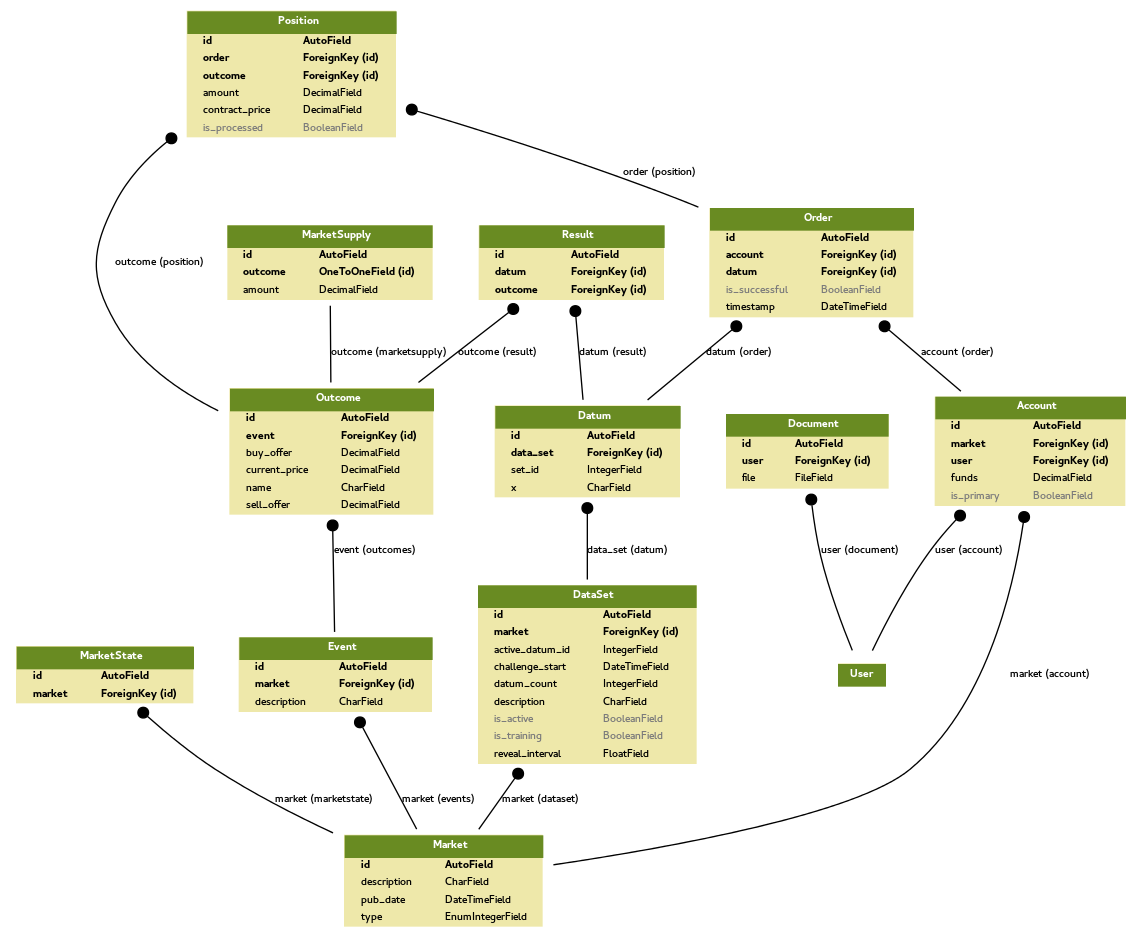
\includegraphics[scale=0.7]{markets_graph.png} }
\label{fig:class_diagram}
\caption{A class diagram of the models comprising the market core. }
\end{figure}


\subsection{Admin Interface}
    The admin interface is the place where market operator can create and configure the hosted markets and manage their contents (in terms of events and data sets) and state.

    Since the framework comes with the built-in {\tt django-admin} module serving this exact purpose, implementing the admin interface was straightforward. Thanks to the aforementioned module, the most common and repetitive operations on models (i.e. create, read, update, delete) were purposefully easy to implement and configure. On the other hand, other less ``popular'' features, such as the option to pre-fill a dataset with randomised entries or to create both an event and its associated outcomes in one go, required carefully reading through the (often quite large) documentation.   

\subsection{API}
    
    Implementing a remote API was one of the more important features of the project in in terms of its intended use as a prediction market framework. Its basic premise is to allow for the development of automated agents that interact with existing markets. While in theory most, if not all, of its functionality mirrors that of the user interface, it is important that the API operates in a secure, well-defined fashion.
    
    I first approached the problem by trying to manually read and write the input in json. Understandably this did not go as expected, even though Django provides both a json serializer and supports simple request handling. 
    
\section{Market Makers}
% talk about the market makers that were or can be implemented.
    What follows is an overview of the created market maker interface and the pricing algorithms investigated in the scope of the project.

\subsection{Interface}
    The two basic actions market makers should provide are processing orders and finalising challenges. Some but not all market makers can additionally provide price quotes. 
    
\subsection{Order Book}
    
    The “city plaza” market scenario where potential buyers and sellers place their offers and the matching ones are resolved. There is normally more than one way to complete trades where for example an agent sells at a price lower than that of a matching buyer, or an agent wishes to buy a larger quantity than a seller has to offer. Usually the market maker is neutral towards both the goods and their prices, but can also be made active by e.g. resolving arbitrage opportunities in his favour.

    Although they are simple to implement and operate, auctions of this type tend to create thin markets with volatile prices and low liquidity of the assets being traded. We can furthermore use the concept of Nash Equilibria to show that such markets do not incentivise players to share their true beliefs and are thus not well suited for model estimation (Myerson et al. 1983). Consider for example a buyer who values a given good well above its current market price: he or she would have no incentive whatsoever to let others (“the market”) know about their high valuation of the good but will instead seek to make trades at the lower price.
    
\subsection{Parimutuel Betting}
This is the system usually used in gambling on sporting events, or in various lotteries. In it all bets of a type are put together in a pool, and the instantaneous odds are determined by the ratios between the already placed bets. The final winnings are determined by sharing the pool (minus any house cuts) amongst the winning bets. Even though they are easy to implement and operate, such markets do not offer any guarantees on the amount that is won in case of success (i.e. the final odds) since the latter is not known until all bets are collected.

This is the only one of the three market makers which was not written in code. 

\subsection{Market Scoring Rule}
In a market scoring rule (MSR) prediction market agents report a probability estimate r on the outcomes of an event and are rewarded sci(r) when outcome i happens. Proper scoring rules are rules which reward estimates close to the truth the highest and penalise estimates that deviate from it, thus incentivising players to act according to their true beliefs.

 [TODO: Review] Such scoring rules are typically monotonically increasing, an example being sci(r)=a+bilog(ri) which is a logarithmic market scoring rule (log-MSR; Hanson, 2002). It is a proper scoring rule which quantifies the risk (also known as self-information in information theory) for the market maker at any time and charges participants proportionally to the change in risk their positions incur: players who move the market prediction towards the “true” distribution (or winning outcomes) get rewarded for doing so, while those who degrade the market prediction are penalised.

In general MSR market schemes are more involved than other examples but also allow for greater flexibility in the pricing strategies.

\section{User Interface}
% mention the static interface, js graphics !!

    As mentioned earlier, adding major features to the user interface was put on hold for the most of the project duration due to a number of concerns. Nonetheless I had a 
    
    There are a few directions I would like to expand on: for example by including histograms to visualise the prices or the trade volume in a market, by allowing browsing other agents’ portfolios, and making the interface more intuitive as a general. A great case study is presented in “A Combinatorial Prediction Market for the U.S. Elections” by Dudik et. al

\section{Other Tools}

\subsection{django-extensions}
    This package is an MIT-licensed collection of extension tools which ease the process of developing Django apps. The two most useful features I used were the ability to automatically generate {\tt django-admin} templates and GraphViz {\tt dot} files of the models in a package. 

\subsection{Sphinx}
    Sphinx is a flexible documentation generator which converts {\tt reStructuredText} (reST) files to a number of formats, most notably PDF and HTML. ReST is a flexible markup language widely used for documentation purposes in the Python community. I was not initially supportive of the idea of learning yet another markup or template language but after looking at possible alternatives Sphinx looked like the most reliable, widely used and {\em pythonic} solution out there. In the end I was able to both quickly generate automatic documentation from the code, and then manually extend and insert additional explanations and use cases for the examples in question.

\section{Testing and Documentation}
% documentation at github.io ?!
% issue tracker ?!?!
% wiki too ?!?!?!?
    When it comes to designing and testing an application dealing with any kind of transactions, it is clear that a set of minimum requirements has to be met in terms of consistency and transactional integrity. Fortunately the high-level nature of the language and the framework make this straightforward.

I initially wanted to adopt a test-driven approach towards the development process but doing so proved hard during  the first few months of the project. During this time I was mainly modelling the market structure and writing code for the front-end. Most of the work was thus of declarative nature and needed little, if any, tests whatsoever. On the other hand Python makes writing runtime validation (i.e. assertions) incredibly easy; a feature I used extensively since the beginning of the project. 

I approached the documentation in a similar manner to testing: while for most of the development process I used the automatically-generated documentation, once I had more-or-less finalised the model designs I started adding custom sections with better explanations. 

\subsection{Unit Tests}

    The main body of unit tests deals with the core market structure and does verification of the basic mechanisms underlying the markets. Example tests include starting, stopping and resetting a dataset or checking if the ``Cron`` module properly dispatches signals whenever markets expire. 
    I took a similar approach when writing the tests for the implemented market maker modules. Currently there are tests only for the {\tt msr-maker} as the other available maker - the order book - is completely neutral. 
    
\subsection{Runtime Tests}
    
    The code features a multitude of runtime tests checking model invariants. For example, the joint asset prices for an outcome space always summing to 1 is enforced throughout the market makers, but there are also explicit checks executed every time prices change.

    While designing the base models, I paid extra attention to transactional atomicity: it would be quite inappropriate if funds appeared or vanished while serving requests in a market. Thankfully the framework allows for fine and idiomatic control of transaction lifetime using method decorators and ``with`` blocks.

\subsection{Documentation}

    The documentation is an integral part of the life-cycle of any software which pretends to be extensible and maintainable, and is especially true in the case of frameworks. While most of the existing documentation is generated automatically, 
    
\subsection{Issues}
    [TODO]
    
\chapter{Evaluation/Reflection}

\section{Functionality}

\section{Interface}

\section{Machine Learning Contests}

\chapter{Conclusion}
% prediction markets and how they can be improved to do even better job
% useful scenarios (e.g. election results, cancer cell detection etc).
% “powerful tool for…”, “excellent alternative to current techniques”




% use the following and \cite{} as above if you use BibTeX
% otherwise generate bibtem entries
\bibliographystyle{unsrt}
\bibliography{ixlib}

\end{document}

